\documentclass{beamer}

\mode<presentation> {
  \usetheme{Warsaw}
  \usecolortheme[rgb={0.37,0.62,0.63}]{structure}

  \setbeamercovered{highly dynamic}
  \usefonttheme{serif}
  \usepackage{ragged2e}
	\justifying
}

\usepackage[spanish]{babel}
\usepackage[utf8]{inputenc}
\usepackage{times}
\usepackage[T1]{fontenc}
\usepackage{amsmath}
\usepackage{amssymb}
\usepackage{verbatim}
\usepackage{hyperref}
\usepackage{xcolor}
\usepackage{booktabs}
\usepackage{tikz}
\usetikzlibrary{arrows.meta,positioning,shapes.geometric,calc}
\usepackage{array}

%%%%%%%%%%%%
\title[35° Simposio Internacional de Estadística]{\textit{\textbf{Nowcasting} del crecimiento económico en Colombia mediante modelos bayesianos de frecuencia mixta}}
%\subtitle{\textit{Evidence from Colombia (2013–2024)}}

\author[Moreno, Olivero y Campo (2026). Nowcasting bayesiano]{Juan Diego Moreno Sánchez \inst{1} \and \and Zeneth Olivero Tapia \inst{2} \\[0.1cm]
\and Jacobo Campo Robledo \inst{1, 2}}
\institute[Universidad Externado de Colombia -- Universidad Católica de Colombia]
{ 
		\inst{1} Universidad Externado de Colombia
%		\and
%		\inst{2} Universidad Católica de Colombia 
		\and 	
		\inst{2} Universidad Católica de Colombia
}

\date{\footnotesize{Julio 14 de 2026}}

\pgfdeclareimage[height=0.4cm]{logo.jpg}{logo}
\logo{\pgfuseimage{logo.jpg}}

\pgfdeclareimage[height=0.4cm]{logo.jpg}{logo}
\pgfdeclareimage[height=0.4cm]{logouex.jpg}{logouex}
%\logo{\pgfuseimage{logo.jpg}}

\setbeamertemplate{sidebar left}
{
\logo{\pgfuseimage{logouex.jpg}}
\vfill
\rlap{\hskip 0.1cm\insertlogo}
\vskip10pt
}

\beamerdefaultoverlayspecification{<+->}


\begin{document}

\begin{frame}
	\titlepage
\end{frame}

\begin{frame}
	\frametitle{Contenido}
	\tableofcontents[pausesections,pausesubsections]
\end{frame}


\section{Introducción - Problema}

\begin{frame}{Introducción - Problema}
\textcolor[rgb]{0,0,1}{\textbf{El Problema del Rezago y la Frecuencia}} 
\begin{itemize}\justifying
    \item \textbf{El Rezago Oficial vs. Nowcasting:} El PIB trimestral es clave para la toma de decisiones, pero el DANE lo publica con $\sim$45 días de rezago. El \textit{nowcasting} soluciona esto estimando el PIB en tiempo real usando un amplio conjunto de variables mensuales (ISE, inflación, petróleo, TRM, etc.). \pause
    \item \textbf{El Problema de la Frecuencia Constante:} Agregar artificialmente los datos mensuales para forzar la estimación de un modelo tradicional puramente trimestral desperdicia el flujo continuo de información y prohíbe actualizar el pronóstico mes a mes. \pause
    \item \textbf{Solución vía Estado Latente:} Se formula un modelo dinámico mensual completo, pero se trata al PIB como un \textbf{\textit{estado latente}} (una variable no observada en 2 de cada 3 meses). Así se resuelve el desfase sin perder ninguna dinámica de alta frecuencia.
\end{itemize}
\end{frame}

\begin{frame}{Introducción - Problema}{¿Por qué un enfoque bayesiano?}
\begin{itemize}\justifying
	\item Un VAR mensual con varias variables y varios rezagos tiene muchos parámetros en relación con el número de observaciones disponibles (\textit{sobreparametrización}) — estimarlo por MV/OLS sin restricciones produce coeficientes muy inestables y sobreajuste. \pause
	\item El enfoque bayesiano permite introducir \textit{priors} de contracción (\textit{shrinkage}), el prior de Minnesota (Litterman, 1986):
	
	\begin{itemize}\justifying
		\item Regulariza los coeficientes hacia una estructura parsimoniosa (ej. paseo aleatorio) sin eliminar variables arbitrariamente
		\item Permite incluir más variables e indicadores de los que un VAR clásico toleraría con series relativamente cortas,
		\item Mejora la precisión fuera de muestra frente a alternativas no restringidas (Bańbura, Giannone y Reichlin (2010)).
	\end{itemize}

\end{itemize}
\end{frame}

\begin{frame}{Introducción - Problema}{¿Por qué un enfoque bayesiano?}
\begin{itemize}\justifying
	\item Además, el marco bayesiano entrega una distribución \textit{posterior} completa del pronóstico (no solo un punto), lo que permite cuantificar la incertidumbre alrededor del \textbf{nowcast} — información valiosa para el análisis de riesgo y la comunicación de política. \pause
	\item El tratamiento de frecuencia mixta (\textit{variable trimestral parcialmente observada}) se resuelve de forma natural dentro de una representación de espacio de estados (\textbf{filtro de Kalman}), que es el marco estándar para inferencia bayesiana en modelos dinámicos.
\end{itemize}
\end{frame}

\begin{frame}{Introducción - Problema}
\begin{block}{Objetivo general}\justifying
Proponer y estimar un modelo de \textit{nowcasting} del crecimiento económico de Colombia mediante un Bayesian Mixed-Frequency VAR (MF-BVAR), que permita actualizar el pronóstico del PIB trimestral a partir de indicadores mensuales de actividad real, precios, condiciones financieras y sector externo.
\end{block}
\end{frame}



\section{Marco Teórico y Revisión de Bibliografía}

\begin{frame}{Marco Teórico y Revisión de Bibliografía}{}
\begin{itemize}\justifying
	\item \textcolor[rgb]{0,0.58,0}{Giannone, Reichlin y Small (2008)}: definen el nowcasting como la actualización continua del pronóstico del trimestre corriente conforme llega nueva información.
	\item \textcolor[rgb]{0.92,0.5,0.4}{Mariano y Murasawa (2003)}: proponen el índice coincidente basado en series mensuales y trimestrales — base de la identidad de agregación en un MF-BVAR.
	\item \textcolor[rgb]{0.92,0.5,0.4}{Kuzin, Marcellino y Schumacher (2011)}: comparan MIDAS vs. VAR de frecuencia mixta para nowcasting del PIB de la eurozona.
	\item \textcolor[rgb]{0.92,0.5,0.4}{Carriero, Clark y Marcellino (2015)}: extienden el MF-BVAR con volatilidad estocástica para pronóstico en tiempo real.
\end{itemize}
\end{frame}

\begin{frame}{Marco Teórico y Revisión de Bibliografía}{}
\begin{itemize}\justifying
	\item \textcolor[rgb]{0,0,1}{Litterman (1986)}: origen del \textit{prior} de Minnesota.
	\item \textcolor[rgb]{0,0,1}{Banbura, Giannone y Reichlin (2010)}: BVAR grandes con contracción — muestran que permite incluir muchas variables sin perder precisión predictiva.
	\item \textcolor[rgb]{0.29,0,0.51}{Schorfheide y Song (2015)}: desarrollan el marco de pronóstico en tiempo real que combina variables mensuales y trimestrales en una estructura VAR de frecuencia mixta.
\end{itemize}
\end{frame}


\section{Datos y Metodología}

\subsection{Datos}

\begin{frame}{Datos}{}\justifying
Se construye un sistema de frecuencia mixta con \textbf{9 variables} para Colombia, combinando una serie trimestral objetivo y ocho indicadores mensuales de actividad real, precios, condiciones monetarias y sector externo. \pause

\begin{table}[h]
\centering
\tiny
\begin{tabular}{llll}
\toprule
\textbf{Variable} & \textbf{Frecuencia} & \textbf{Fuente} & \textbf{Rol} \\
\midrule
PIB real & Trimestral & DANE & Variable objetivo \\
ISE & Mensual & DANE & Actividad económica agregada \\
IPI (Producción industrial) & Mensual & DANE & Sector manufacturero \\
Tasa de desempleo & Mensual & DANE & Mercado laboral \\
Inflación (IPC) & Mensual & DANE & Precios \\
TRM & Mensual & Banco de la República & Sector externo / financiero \\
Tasa de política monetaria & Mensual & Banco de la República & Condiciones monetarias \\
Petróleo (Brent) & Mensual & Mercados internacionales & Choque externo (términos de intercambio) \\
IEC & Mensual & Fedesarrollo & Expectativas \\
\bottomrule
\end{tabular}
\end{table}
\end{frame}

\begin{frame}{Datos}{Muestra y Transformaciones}\justifying
\begin{itemize}\justifying
    \item \textbf{Muestra histórica}: 2014--2026 (hasta Abril).
    \item \textbf{Muestra de nowcasting}: 2021--2026 (submuestra reciente, usada para el ejercicio de pronóstico en tiempo real).
    \item Todas las series mensuales se emplean desestacionalizadas.
    \item Las variables se modelan \textbf{en niveles}; la no estacionariedad se controla directamente a través del \textit{prior} de Minnesota, que impone la hipótesis de \textit{random walk} sobre el primer rezago propio de cada variable.
\end{itemize}
\end{frame}


\subsection{Metodología}

\begin{frame}{Metodología}{Panorama General}\justifying
El modelo se estima en tres etapas: \pause
\begin{enumerate}\justifying
    \item \textbf{Especificación}: VAR mensual en forma de espacio de estados, con el PIB trimestral como variable parcialmente observada (Schorfheide y Song, 2015). \pause
    \item \textbf{Estimación bayesiana}: muestreador de Gibbs, combinando simulación de estados (Carter-Kohn, 1994) y actualización de parámetros bajo \textit{prior} de Minnesota. \pause
    \item \textbf{Proyección}: densidad predictiva conjunta del PIB mensual latente, agregada de forma consistente al horizonte trimestral de interés.
\end{enumerate}
\end{frame}

\begin{frame}{Metodología}{Dinámica del Sistema (Ecuación de Transición)}\justifying
Sea $x_t = [x_{m,t}', x_{q,t}']'$ un vector $n \times 1$ de variables macroeconómicas. La dinámica mensual evoluciona según un proceso autorregresivo: \pause
\[
Z_t = F(\Phi) Z_{t-1} + F_c(\Phi) + V_t, \quad V_t \sim \text{i.i.d. } N(0, \Omega(\Sigma))
\] \pause
Donde la matriz compañera $F(\Phi)$ y la matriz singular de covarianza $\Omega(\Sigma)$ asimilan los rezagos del sistema original: \pause
\[
F(\Phi) = \begin{bmatrix} \Phi_1 & \Phi_2 & \dots & \Phi_p \\ I_{n(p-1)} & & 0_{n(p-1) \times n} \end{bmatrix}, \quad \Omega(\Sigma) = \begin{bmatrix} \Sigma & 0 \\ 0 & 0 \end{bmatrix}
\]
\end{frame}

\begin{frame}{Metodología}{Ecuación de Medición y Restricción Aditiva}\justifying
Para relacionar el vector mensual latente con los datos oficiales y solucionar el problema de desfase de publicación (\textit{ragged edge}): \pause
\[
Y_t^{obs} = M_t \Lambda Z_t
\] \pause
Donde $M_t$ es una matriz variante en el tiempo que apaga las celdas vacías (NA) en el mes $t$, y $\Lambda$ es la matriz de agregación temporal. \pause \\ \vspace{0.3cm}
\textbf{Restricción Aditiva del PIB} \\
Como el PIB se modela en niveles, la agregación trimestral impone una restricción determinística en el Filtro de Kalman: \pause
\[
PIB_{Q, t} = PIB_{M, t}^* + PIB_{M, t-1}^* + PIB_{M, t-2}^*
\]
\end{frame}

\begin{frame}{Metodología}{Muestreo de Gibbs (Simulación de Estados y Parámetros)}\justifying
La estimación del modelo iterará 20,000 veces sobre dos pasos: \pause
\begin{enumerate}\justifying
    \item \textbf{Simulación de Estados (Carter-Kohn, 1994)}: Sorteo de la trayectoria $Z_{1:T}$ condicionado a los parámetros fijos: \pause
    \[
    p(Z_{1:T} \mid Y_{1:T}^{obs}, \Phi, \Sigma) \propto p(Z_0) \prod_{t=1}^T p(Y_t^{obs} \mid Z_t) p(Z_t \mid Z_{t-1}, \Phi, \Sigma)
    \] \pause
    \item \textbf{Simulación de Parámetros (\textit{Prior} de Minnesota)}: Sorteo de $(\Phi, \Sigma)$ condicionado al vector de estados simulado: \pause
    \[
    p(\Phi, \Sigma \mid Y_{1:T}^{obs}, Z_{1:T}) \sim MNIW(\bar{\Phi}, \bar{\Psi}, \bar{\Sigma}, \bar{\nu})
    \]
\end{enumerate}
\end{frame}

\begin{frame}{Metodología}{Pronóstico: Densidad Predictiva Posterior}\justifying
Finalmente, en el horizonte de pronóstico $T+1, \dots, T+H$, el PIB mensual latente se proyecta marginalizando la incertidumbre: \pause
\[
p(Z_{T+1:T+H} \mid Y_{1:T}^{obs}) = \int p(Z_{T+1:T+H} \mid Z_T, \Phi, \Sigma) p(\Phi, \Sigma \mid Datos) \, d(\Phi, \Sigma)
\] \pause \\ \vspace{0.3cm}
\begin{itemize}
    \item Esta integral se aproxima mediante el remuestreo de las trayectorias de Montecarlo (descartando el \textit{burn-in}).
    \item Genera estimaciones puntuales (la mediana) y bandas de incertidumbre o credibilidad (ej. 95\%).
\end{itemize}
\end{frame}

\begin{frame}{Metodología}{Calibración y Diagnósticos de Convergencia MCMC}
\begin{itemize}\justifying
    \item \textbf{Prior de Minnesota}: $\lambda_1 = 0.09$. Controla la contracción de los coeficientes hacia la hipótesis de \textit{random walk} en cada variable.
    \item \textbf{Simulaciones}: 20{,}000 (\textit{draws}), 10{,}000 calentamiento (\textit{burn-in}).
    \item \textbf{Especificación de rezagos}: $p=6$ en la muestra histórica completa; $p=4$ en la submuestra de nowcasting (2021--2026), para evitar singularidad en la matriz de covarianza del prior.
    \item \textbf{Tamaño de muestra efectivo (ESS)}:
    \begin{itemize}\justifying
        \item Muestra histórica ($p=6$): ESS $= 3{,}989.74$
        \item Muestra de nowcasting ($p=4$): ESS $= 1{,}914.61$
    \end{itemize}
    \item Un ESS alto (\textit{relativo}) indica baja autocorrelación en la cadena y buena mezcla del muestreador de Gibbs (convergencia adecuada).
\end{itemize}
\end{frame}


\section{Estimaciones y Resultados}

\begin{frame}{Estimaciones y Resultados}{Pronóstico para el Segundo Trimestre de 2026 (Q2)}\justifying
Proyección del modelo MF-BVAR para el trimestre evaluado: \\[0.2cm] \pause
\begin{table}[h]
\centering
\scriptsize
\begin{tabular}{lccc}
\toprule
\textbf{Métrica / Indicador} & \textbf{Mediana BVAR} & \textbf{Intervalo de Credibilidad (95\%)} \\
\midrule
PIB real (niveles, MM) & \textbf{262,181.0} & [256,930.0 \text{ a } 267,471.0] \\
Crec. Intertrimestral (Q2 vs Q1-2026) & \textbf{+1.31\%} & [-0.72\% \text{ a } +3.36\%] \\
Crec. Interanual (Q2-2026 vs Q2-2025) & \textbf{+3.48\%} & [+1.41\% \text{ a } +5.57\%] \\
\bottomrule
\end{tabular}
\end{table} \vspace{0.2cm} \pause
Se estima un crecimiento intertrimestral del \textbf{+1.31\%} y un crecimiento interanual del \textbf{+3.48\%} para el Q2-2026.
\end{frame}

\begin{frame}{Estimaciones y Resultados}{Pronóstico del PIB Mensual Latente (Abril-Junio 2026)}\justifying
Desagregación del pronóstico trimestral en sus componentes mensuales latentes estimados por el Filtro de Kalman: \vspace{0.2cm} \pause
\begin{table}[h]
\centering
\scriptsize
\begin{tabular}{lccc}
\toprule
\textbf{Mes Proyectado} & \textbf{Mediana BVAR} & \textbf{Límite Inf (95\%)} & \textbf{Límite Sup (95\%)} \\
\midrule
Abril 2026 & \textbf{86,458.1} & 84,950.0 & 87,950.0 \\
Mayo 2026 & \textbf{86,862.3} & 85,050.0 & 88,600.0 \\
Junio 2026 & \textbf{88,860.6} & 86,930.0 & 90,921.0 \\
\bottomrule
\end{tabular}
\end{table} \vspace{0.2cm} \pause
La suma de estos tres meses resulta en la estimación del trimestre agregado (262,181.0), validando la restricción de medición del modelo.
\end{frame}

\begin{frame}{Estimaciones y Resultados}{Importancia Predictiva de las Variables}
Para entender de dónde provienen las mayores ganancias de información en el pronóstico del PIB latente, se calculó la \textbf{Descomposición Histórica de la Varianza del Error de Pronóstico (FEVD)} a 12 meses:\\[0.3cm]
\textbf{Aporte a la varianza predictiva del PIB:} \pause
\begin{itemize}
    \item \textbf{Índice de Seguimiento a la Economía (ISE):} \textcolor{blue}{23.06\%}
    \item \textbf{Tasa de Intervención (BanRep):} \textcolor{blue}{16.83\%}
    \item \textbf{Índice de Confianza del Consumidor (ICC):} \textcolor{blue}{14.45\%}
    \item \textbf{Tasa de Desempleo (TD):} \textcolor{blue}{12.54\%}
    \item \textbf{Precio del Petróleo (Brent):} \textcolor{blue}{11.04\%}
\end{itemize}
\end{frame}

\begin{frame}{Estimaciones y Resultados}{PIB Mensual Latente Completo}
\begin{center}
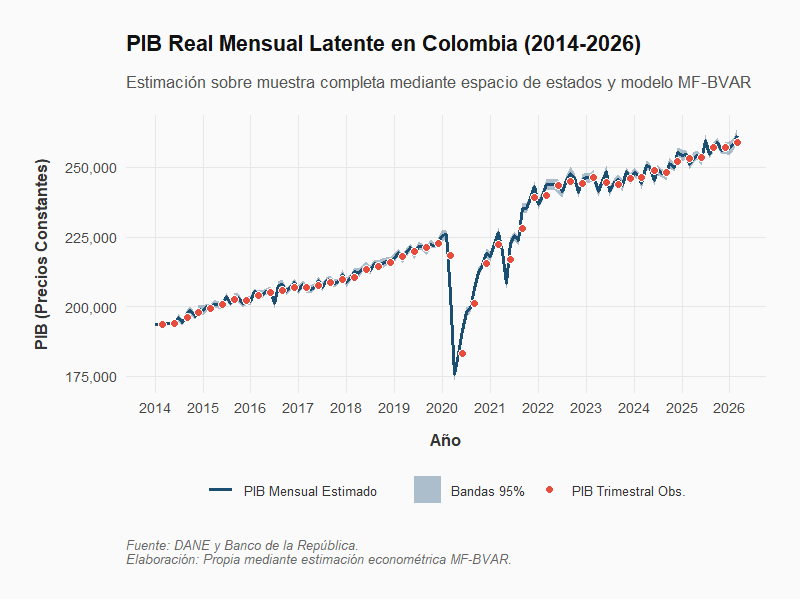
\includegraphics[width=0.95\textwidth,height=0.8\textheight,keepaspectratio]{pib_mensual_latente_completo.png}
\end{center}
\end{frame}

\begin{frame}{Estimaciones y Resultados}{Pronóstico Trimestral Q2-2026}
\begin{center}
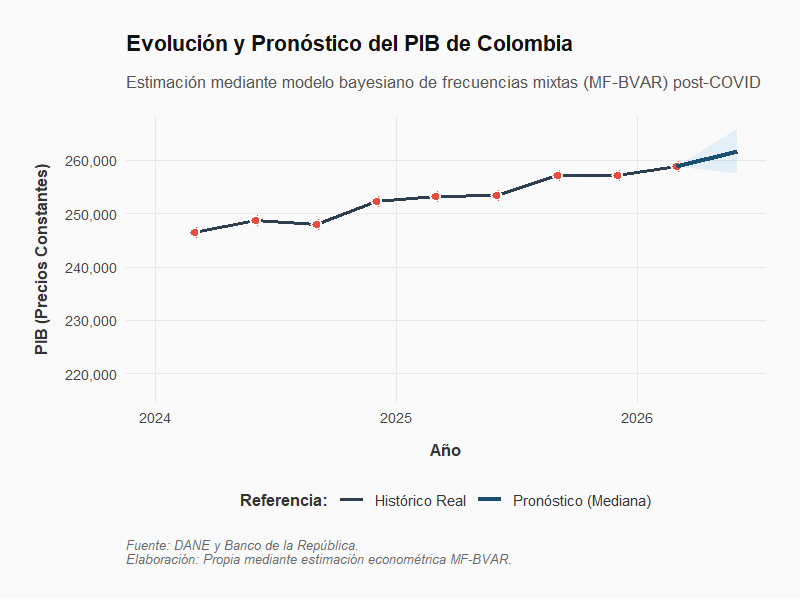
\includegraphics[width=0.95\textwidth,height=0.8\textheight,keepaspectratio]{pib_trimestral_pronostico.png}
\end{center}
\end{frame}



\section{Consideraciones finales}

%\begin{frame}{Consideraciones finales}{}\justifying
%\begin{block}{ }\justifying

%\end{block}
%\pause
%\begin{itemize}\justifying
%	\item 
%	\item 
%\end{itemize}
%\end{frame}

\begin{frame}{Consideraciones finales}{}
\begin{itemize}\justifying
    \item El MF-BVAR permite generar \textbf{nowcasts mensuales del PIB colombiano} explotando la información disponible antes de la publicación oficial trimestral del DANE, sin sacrificar la coherencia estadística entre frecuencias. \pause
    \item El tratamiento del PIB como \textbf{variable de estado latente} --- y no como un dato interpolado mecánicamente --- permite que la agregación trimestral opere como una restricción de medición exacta dentro del filtro de Kalman. 
\end{itemize}
\end{frame}

\begin{frame}{Consideraciones finales}{}
\begin{itemize}\justifying
    \item Las proyecciones revelan un crecimiento esperado interanual del \textbf{3.48\%} para el segundo trimestre de 2026, lo que demuestra la utilidad del MF-BVAR para anticipar escenarios económicos con base en información adelantada. \pause
    \item El enfoque bayesiano (prior de Minnesota + MNIW) resuelve el problema de sobreparametrización inherente a un VAR mensual con múltiples variables y rezagos, permitiendo estimar el sistema incluso con series relativamente cortas.
\end{itemize}
\end{frame}

\begin{frame}{}\justifying
\begin{block}{}
\begin{center}
\huge{\textbf{MUCHAS GRACIAS...!}}
\end{center}
\end{block}
\end{frame}

\end{document}
